\fontfamily{\sfdefault}\selectfont
% XCircuit output "loop_bandwidth.tex" for LaTeX input from loop_bandwidth.ps
\def\putbox#1#2#3#4{\makebox[0.00000in][l]{\makebox[#1][l]{}\raisebox{\baselineskip}[0.00000in][0.00000in]{\raisebox{#2}[0.00000in][0.00000in]{\scalebox{#3}{#4}}}}}
\def\rightbox#1{\makebox[0.00000in][r]{#1}}
\def\centbox#1{\makebox[0.00000in]{#1}}
\def\topbox#1{\raisebox{-0.60\baselineskip}[0.00000in][0.00000in]{#1}}
\def\midbox#1{\raisebox{-0.20\baselineskip}[0.00000in][0.00000in]{#1}}
   \scalebox{1}{
   \normalsize
   \parbox{2.83854in}{
   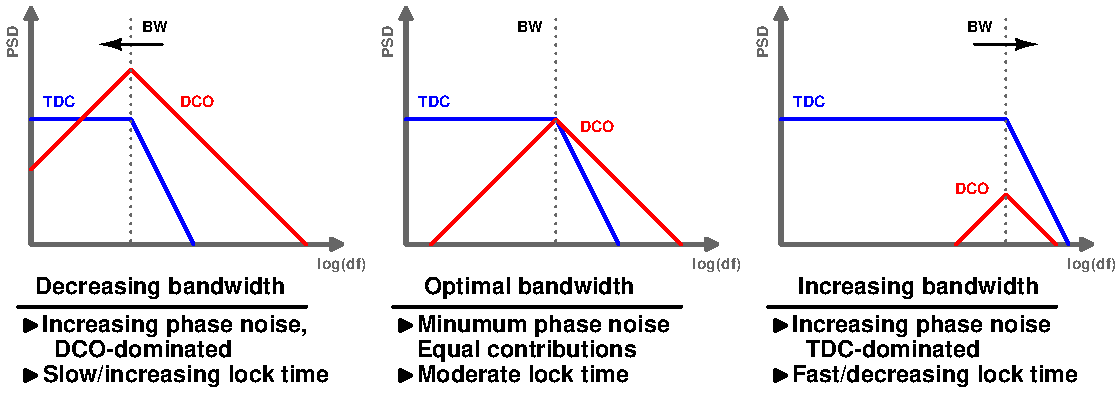
\includegraphics[scale=1.00000]{./figs/loop_bandwidth.pdf}\\
   % translate x=-296 y=227 scale 0.38
   \putbox{2.18000in}{0.07000in}{0.60}{$\log(\Delta f)$}%
   \putbox{0.06000in}{1.74000in}{0.60}{PSD}%
   \putbox{0.72000in}{1.49000in}{0.60}{-30 dB/dec}%
   \putbox{0.72000in}{1.36000in}{0.60}{$\propto f^{-3}$}%
   \putbox{1.39000in}{0.90000in}{0.60}{$\propto f^{-2}$}%
   \putbox{1.39000in}{1.03000in}{0.60}{-20 dB/dec}%
   \putbox{0.76000in}{0.11000in}{0.60}{\rotatebox{-360}{$f_1$}}%
   \putbox{1.76000in}{0.11000in}{0.60}{\rotatebox{-360}{$f_2$}}%
   } % close 'parbox'
   } % close 'scalebox'
   \vspace{-\baselineskip} % this is not necessary, but looks better
\fontfamily{\rmdefault}\selectfont
